% Problem description
Coupling single-mode fibers to waveguides with the help of microlenses is a very common setup in integrated optics \cite{integrated_optics}. Because a lensed fiber has a minimum focal length, by means of this technique simple and reliable optical systems with a small size become possible. In this work the implementation of the lensed fiber-to-chip will be discussed and its coupling efficiency will be investigated.\\

\begin{figure}[!ht]
\centering
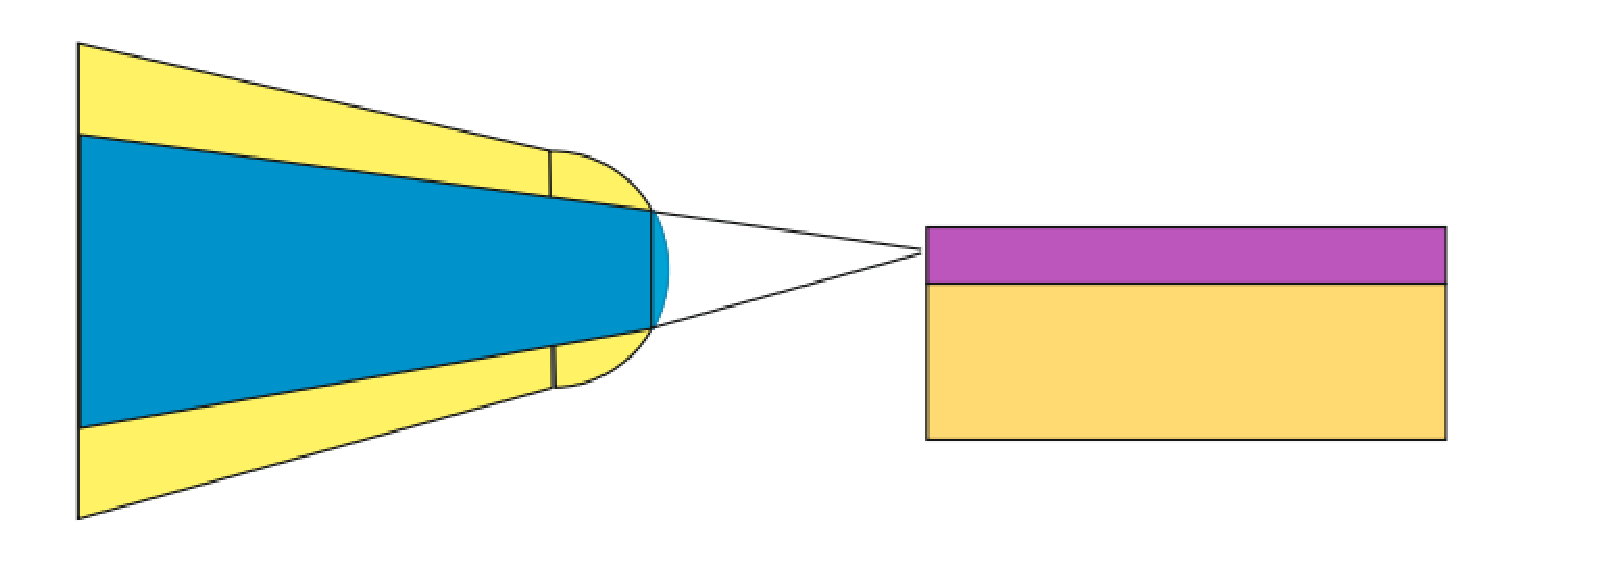
\includegraphics[width=.7\textwidth]{bilder/experiment_object}
\caption{Fiber-to-Chip interface.}
\label{fig:experiment_object}
\end{figure}
Fig. \ref{fig:experiment_object} shows a schematic fiber-to-chip interface. At the one side there is a lensed tapered fiber as laser source and at another side there is a rib waveguide\cite{integrated_optics}, located at the working distance of the fiber, as the signal receiver.\\
 
\begin{figure}[!ht]
\centering
\subfigure[Picture of a real Single mode lensed fiber\cite{nanoscal_tapered_fiber}.]{
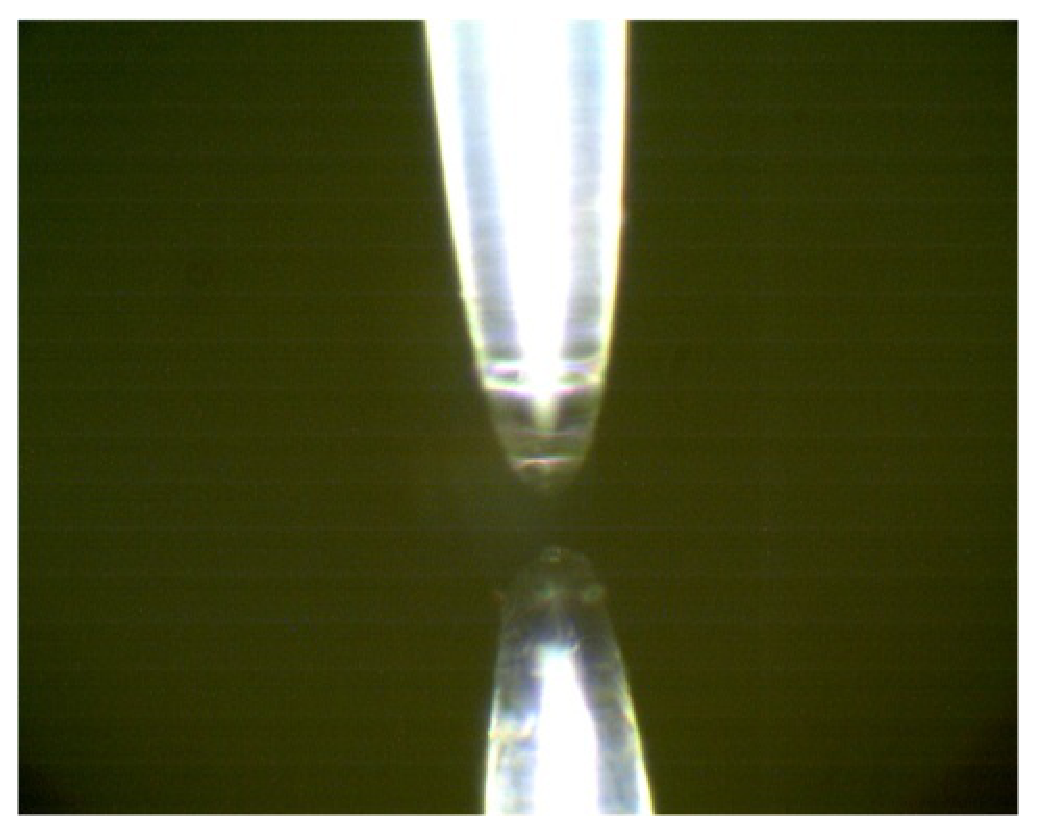
\includegraphics[width=0.3\textwidth]{bilder/single_mode_lensed_fibber}
\label{fig:single_mode_lensed_fiber}
}
\hfill
\subfigure[Schema of a tapered lensed fiber\cite{nanoscal_tapered_fiber}.]{
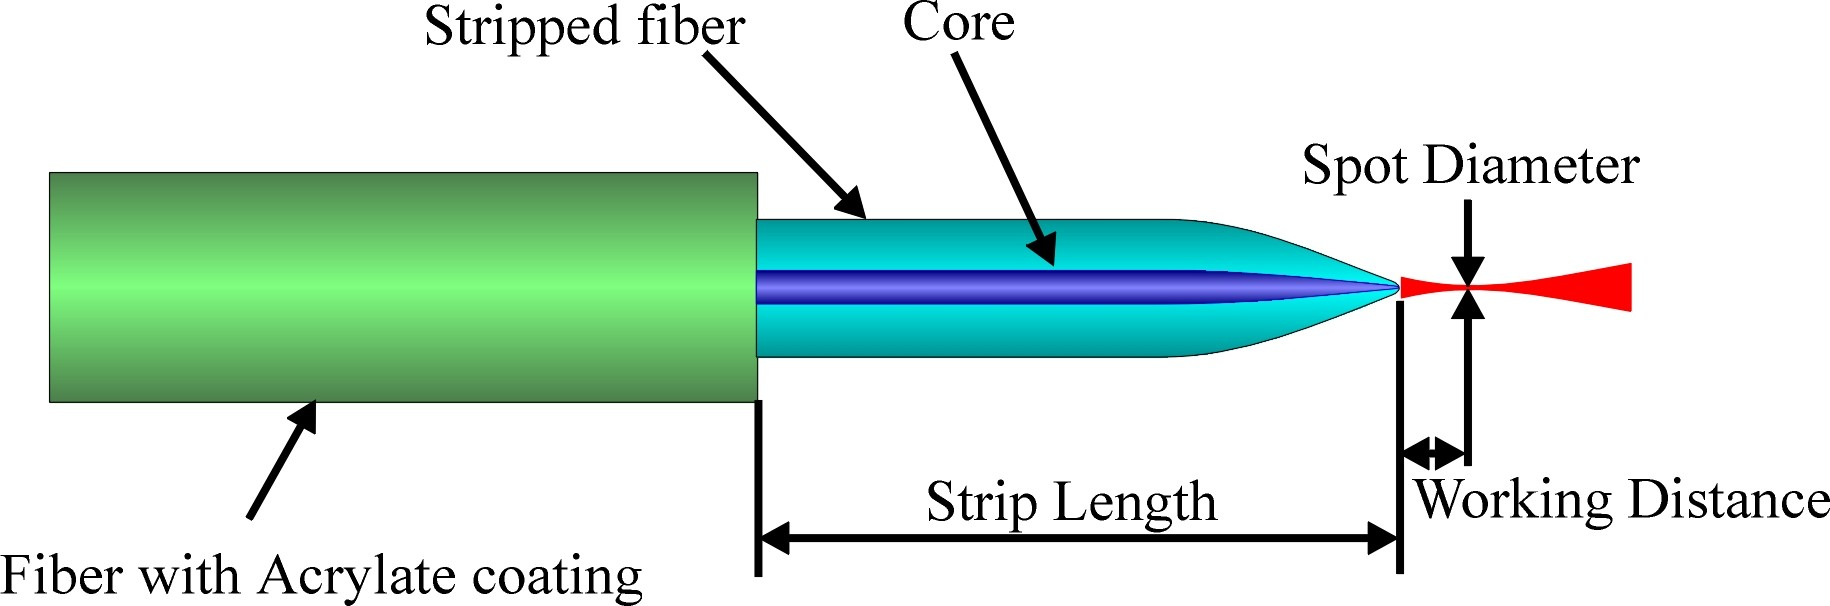
\includegraphics[width=0.6\textwidth]{bilder/tapered_lensed_fiber}
\label{fig:tapered_lensed_fiber}
}
\label{fig:TLFs}
\caption{ Tapered and Lensed Fibers by NANOICS.}
\end{figure}
In the experimental setup for this work tapered lensed fibers from NANONICS\cite{nanoscal_tapered_fiber} are used. Fig. \ref{fig:single_mode_lensed_fiber} shows the photograph of the tapered fiber by NANONICS and Fig. \ref{fig:tapered_lensed_fiber} indicates its schema. In Tab. \ref{tab:technical parameters_lensed_fiber} parts of technical parameters are listed. Additional information about the experimental setup is that the working wavelength is $\lambda=1064$nm ($f=282$THz) and working distance $4\mu$m.\\
 
\begin{table}[!ht]
\caption{Technical parameters about tapered lensed fiber\cite{nanoscal_tapered_fiber}.}
\begin{tabular}{|c|c|c|}
\hline
\multicolumn{2}{|c|}{\textbf{Parameter}}&\textbf{Specification(Single-Mode)}\\
\hline
\multirow{3}{*}{\parbox[c]{0.25\textwidth}{Spot Size of Aspheric and Convex Lenses ($1/e^2$)}
}&\multirow{2}{*}{Minum}&$1.7\mu$m($\lambda=1.5\mu$m)\\
&																		 &$0.6\mu$m($\lambda=0.6\mu$m)\\
\cline{2-3}
&Maxium															 &$6.0\mu$m($\lambda=1.5\mu$m)\\
\hline
\multirow{2}{*}{Spot Size Tolerance}&\parbox[c]{0.25\textwidth}{
\begin{center}
Without near-field characterization
\end{center}
} & $\pm 0.5\mu$m\\
\cline{2-3}
&\parbox[c]{0.25\textwidth}{
\begin{center}
With near-field characterization
\end{center}
} &$ \pm 0.25\mu$m\\
\hline
\multirow{2}{*}{Working Distance} &Minimum &$5\mu$ m($\lambda=1.5\mu$m)\\
\cline{2-3}
&																	Maximum &$50\mu$ m($\lambda=1.5\mu$m)\\
\hline
\end {tabular}
\label{tab:technical parameters_lensed_fiber}
\end{table}

\begin{figure}[!ht]
\centering
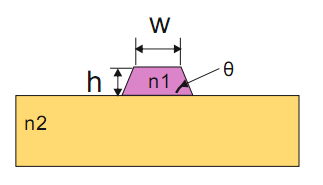
\includegraphics[width=0.6\textwidth]{bilder/orignial_waveguide}
\caption{Schema of the photonic waveguide.}
\label{fig:photonic_waveguide}
\end{figure}
Actually, the waveguide in experimental setup is a trapezoid guide on a semiconductor like Fig. \ref{fig:photonic_waveguide}. The angles $\theta$ of this guide approximate to $90^{o}$ and is not easy to measure because of the micro-size of the structure. Thus a simplified guide model with $\theta=90^{o}$ will be used in this work. The detailed technical properties of the photonic waveguide used in the experimental setup are given as following:
\begin{itemize}
\item Working wavelength: $\lambda=1064$nm
\item Waveguide: LiNbO$_{3}$ with $n_{1}=2.516, w\approx 1\mu$m, $h\approx 0.5 \mu$m
\item Substrate: SiO$_{2}$ with $n_{2}=1.544 $
\end{itemize}
